\begin{pastexam}[label={px:gw3-114-ds-01}]{關務三等資訊處理 114 年 第一題}
（申論；25 分）

給予一前序（preorder）表示式 ABCD 和後序（postorder）表示式 DCBA，試畫出所有可能的二元樹。（25 分）
\end{pastexam}

\begin{pastsoln}
\textbf{答案：共 $8$ 棵}，都是一條直鏈 $A - B - C - D$，差別在每一步往左還是往右。

\textbf{推理。} 前序是「根、左子樹、右子樹」，後序是「左子樹、右子樹、根」。
\begin{enumerate}[nosep]
\item 前序第一個、後序最後一個都是 $A$，$A$ 是根；剩下的前序 $BCD$、後序 $DCB$ 是 $A$ 的子樹部分。
\item 若 $A$ 有左、右兩棵非空子樹，前序 $A$ 之後的第一個 $B$ 是左子樹的根；左子樹在後序裡排在最前面，
而且以它的根 $B$ 結尾，所以左子樹就是後序從頭到 $B$ 的 $\{D, C, B\}$，右子樹是空的，矛盾。 所以
$A$ 只有一個子節點 $B$，但\textbf{前序和後序都分不出它在左邊還是右邊}：$B$ 當左子或右子，前序都是
$A$ 接著 $B$ 的子樹、後序都是 $B$ 的子樹接著 $A$。
\item 對 $B$ 的子樹（前序 $BCD$、後序 $DCB$）同樣推理：$B$ 只有一個子節點 $C$，左右都可以；$C$ 只有一個
子節點 $D$，左右都可以；$D$ 是葉節點。
\end{enumerate}
三個子節點 $B$、$C$、$D$ 各有左、右兩種放法，共 $2^3 = 8$ 棵。 這也說明了只給前序和後序一般不能唯一決定
二元樹：每個「只有一個子節點」的節點都會產生左右兩種可能（資結書第~7.4~節、定理~7.5）。

下圖每棵樹下方的三個字母依序表示 $B$、$C$、$D$ 是父節點的左子（L）或右子（R）：
\begin{center}
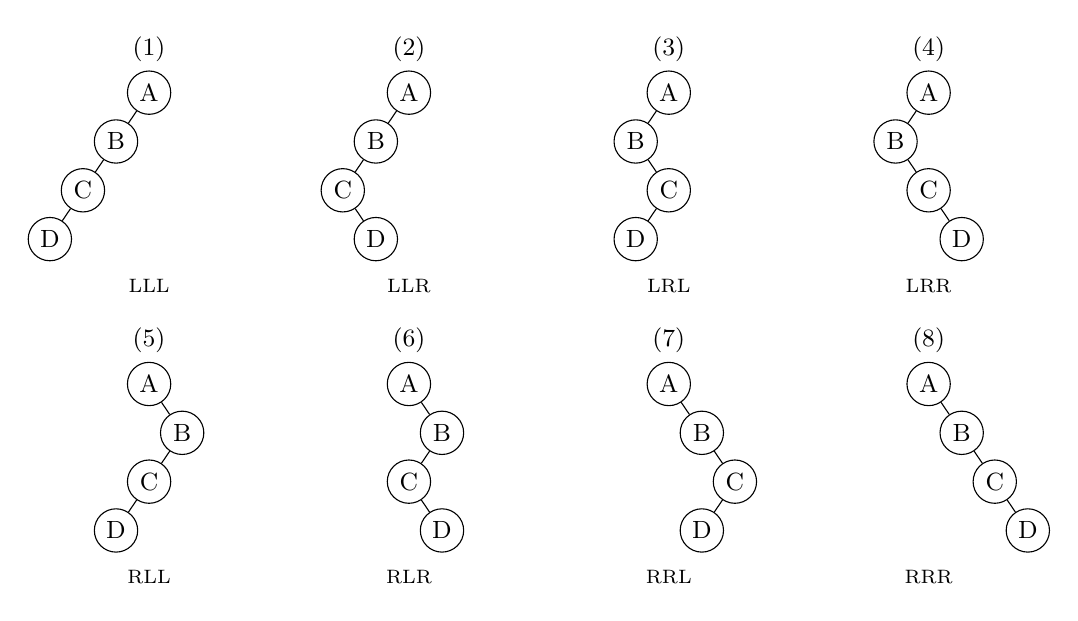
\begin{tikzpicture}[v/.style={circle, draw, minimum size=5.5mm, inner sep=0pt, font=\small}]
\begin{scope}[xshift=0.0cm, yshift=0.0cm]
\node[font=\small] at (0,0.55) {(1)};
\node[v] (A0) at (0.00,0.00) {A};
\node[v] (B0) at (-0.42,-0.62) {B};
\node[v] (C0) at (-0.84,-1.24) {C};
\node[v] (D0) at (-1.26,-1.86) {D};
\draw (A0)--(B0)--(C0)--(D0);
\node[font=\scriptsize] at (0,-2.45) {LLL};
\end{scope}
\begin{scope}[xshift=3.3cm, yshift=0.0cm]
\node[font=\small] at (0,0.55) {(2)};
\node[v] (A1) at (0.00,0.00) {A};
\node[v] (B1) at (-0.42,-0.62) {B};
\node[v] (C1) at (-0.84,-1.24) {C};
\node[v] (D1) at (-0.42,-1.86) {D};
\draw (A1)--(B1)--(C1)--(D1);
\node[font=\scriptsize] at (0,-2.45) {LLR};
\end{scope}
\begin{scope}[xshift=6.6cm, yshift=0.0cm]
\node[font=\small] at (0,0.55) {(3)};
\node[v] (A2) at (0.00,0.00) {A};
\node[v] (B2) at (-0.42,-0.62) {B};
\node[v] (C2) at (0.00,-1.24) {C};
\node[v] (D2) at (-0.42,-1.86) {D};
\draw (A2)--(B2)--(C2)--(D2);
\node[font=\scriptsize] at (0,-2.45) {LRL};
\end{scope}
\begin{scope}[xshift=9.899999999999999cm, yshift=0.0cm]
\node[font=\small] at (0,0.55) {(4)};
\node[v] (A3) at (0.00,0.00) {A};
\node[v] (B3) at (-0.42,-0.62) {B};
\node[v] (C3) at (0.00,-1.24) {C};
\node[v] (D3) at (0.42,-1.86) {D};
\draw (A3)--(B3)--(C3)--(D3);
\node[font=\scriptsize] at (0,-2.45) {LRR};
\end{scope}
\begin{scope}[xshift=0.0cm, yshift=-3.7cm]
\node[font=\small] at (0,0.55) {(5)};
\node[v] (A4) at (0.00,0.00) {A};
\node[v] (B4) at (0.42,-0.62) {B};
\node[v] (C4) at (0.00,-1.24) {C};
\node[v] (D4) at (-0.42,-1.86) {D};
\draw (A4)--(B4)--(C4)--(D4);
\node[font=\scriptsize] at (0,-2.45) {RLL};
\end{scope}
\begin{scope}[xshift=3.3cm, yshift=-3.7cm]
\node[font=\small] at (0,0.55) {(6)};
\node[v] (A5) at (0.00,0.00) {A};
\node[v] (B5) at (0.42,-0.62) {B};
\node[v] (C5) at (0.00,-1.24) {C};
\node[v] (D5) at (0.42,-1.86) {D};
\draw (A5)--(B5)--(C5)--(D5);
\node[font=\scriptsize] at (0,-2.45) {RLR};
\end{scope}
\begin{scope}[xshift=6.6cm, yshift=-3.7cm]
\node[font=\small] at (0,0.55) {(7)};
\node[v] (A6) at (0.00,0.00) {A};
\node[v] (B6) at (0.42,-0.62) {B};
\node[v] (C6) at (0.84,-1.24) {C};
\node[v] (D6) at (0.42,-1.86) {D};
\draw (A6)--(B6)--(C6)--(D6);
\node[font=\scriptsize] at (0,-2.45) {RRL};
\end{scope}
\begin{scope}[xshift=9.899999999999999cm, yshift=-3.7cm]
\node[font=\small] at (0,0.55) {(8)};
\node[v] (A7) at (0.00,0.00) {A};
\node[v] (B7) at (0.42,-0.62) {B};
\node[v] (C7) at (0.84,-1.24) {C};
\node[v] (D7) at (1.26,-1.86) {D};
\draw (A7)--(B7)--(C7)--(D7);
\node[font=\scriptsize] at (0,-2.45) {RRR};
\end{scope}
\end{tikzpicture}
\end{center}
檢查其中一棵，例如 (2) LLR：$A$ 的左子 $B$，$B$ 的左子 $C$，$C$ 的右子 $D$。 前序：$A, B, C, D$；後序：
先走 $A$ 的左子樹，$B$ 的左子樹，$C$ 的（空）左子樹、右子樹 $D$，再 $C$、$B$、$A$，得 $D, C, B, A$，
符合。 其餘七棵同理。
\end{pastsoln}
